\documentclass{article}
\usepackage[a4paper, total={6in, 8in}]{geometry}
\usepackage{graphicx}
\usepackage{url}
\usepackage{natbib}
\usepackage{todonotes}
\usepackage{booktabs}
\usepackage{lineno}


\linespread{2}

% Title
\title{A Topic Model of Climate Change Literature}
\title{Words, words, words: Mapping the Matter of Climate Change Literature}
\title{A Topography of Climate Change Research}
%\author{Max Callaghan}


\begin{document}
\maketitle

\linenumbers

\textbf{
To contribute to evidence-based policies on tackling climate change, the IPCC aims to comprehensively assess the relevant scientific literature \citep{IPCC2013}. With the size of this literature currently almost two orders of magnitude larger than at the time of the IPCC's first assessment report, this task has become impossible without the aid of machine-reading. We collect over 400,000 abstracts from Web of Science (WoS) and Scopus, and develop a topic model in order to give an overview of this unmanageably large corpus. This overview shows us the distribution and development of topics across the literature, and allows us to identify topics with greater and lesser representation in IPCC reports. %[We find that new topics, such as [biochar] can be identified as they emerge, an application with a high potential for increasing the relevance and comprehensiveness of future IPCC assessments.]
}

\begin{figure}
\begin{center}
	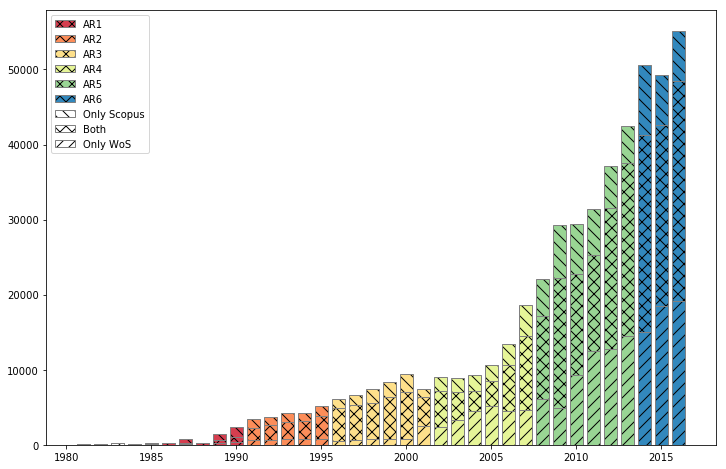
\includegraphics[width=0.8\linewidth]{plots/wos_scopus_docs_time}
    \caption{Growth in relevant literature in WoS and Scopus}
    \label{growth}
    \end{center}
\end{figure}

The size of the scientific literature on climate change has expanded rapidly over the lifetime of the IPCC. While the first assessment report had around 5,500 articles to assess, nearly 5,000 new articles are now published every month, bringing the total size of the literature to close to half a million papers, (Figure \ref{growth}).  The increase in volume, velocity, and variety of content to be assessed has turned the task of the IPCC into a `Big Literature' challenge \citep{Minx2017BigChange}. To ask questions about the literature \textit{at scale}, we now need to apply computational techniques to the analysis of large document collections.

Topic models are one such technique. A topic model learns the latent topics that structure a large corpus of documents, by leveraging the systematic co-occurrence of words across documents. Topics are distributions of words, and the topic mixture of each document explains the words observed in that document. This means that topic models can aid the understanding of large corpuses, and of the place of individual documents within them, by showing a document or corpus as a combination of 100 or so intelligible topics, rather than combinations of thousands of words.

Assessment-makers like the IPCC have been described as cartographers for policymakers \citep{Edenhofer2015}. As such their purpose is, summarising available scientific knowledge, to describe the problem and solution space of a policy issue. The topic model presented here is a rough map of climate change research since 1985. It shows a broad outline of the topics that make up this research and how they relate to each other, and demonstrates how this has changed over time. Such a map sheds light on the terrain of knowledge about a policy issue, making an overview of an unmanageably large and diverse landscape possible. This overview allows both for the production of policy pathways that are well informed by science, and, as demonstrated in this paper, the assessment of the comprehensiveness with which these pathways reflect the landscape.




While topic modelling has been employed to answer specific questions about small aspects of climate literature, e.g. \citep[e.g.][]{Minx2017FastEmissions, Grubert2016}, this is the first application of topic models to gain an overview of the entire field.









\section*{Results}

\todo{From here on in, the paper is more of an outline, with a mixture of bullet points about results that exist or I would still like to generate}

\begin{figure}
\begin{center}
	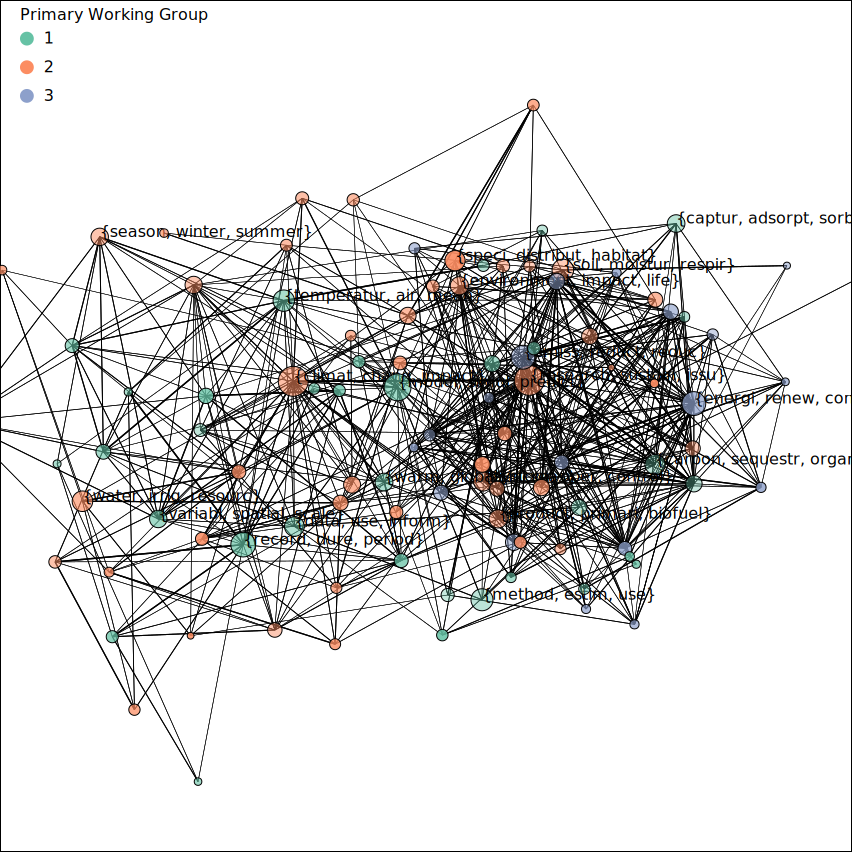
\includegraphics[width=0.8\linewidth]{plots/network_wg_65}
    \caption{Topic structure of climate change literature}
    \label{network}
    \end{center}
\end{figure}

\subsection*{Topic Model}
\begin{itemize}
	\item Figure \ref{network} shows the structure of the topic model with 100 topics, with each node coloured according to the IPCC working group in which the highest proportion of the topic's documents are cited.
    \item Topics that systematically co-occur in documents are linked, and the resulting network is displayed with links weighted according to topic correlation score. The strength of links is greater where two topics are categorised as being in the same working group. This relationship is statistically significant (see SI)
\end{itemize}

\begin{figure}
	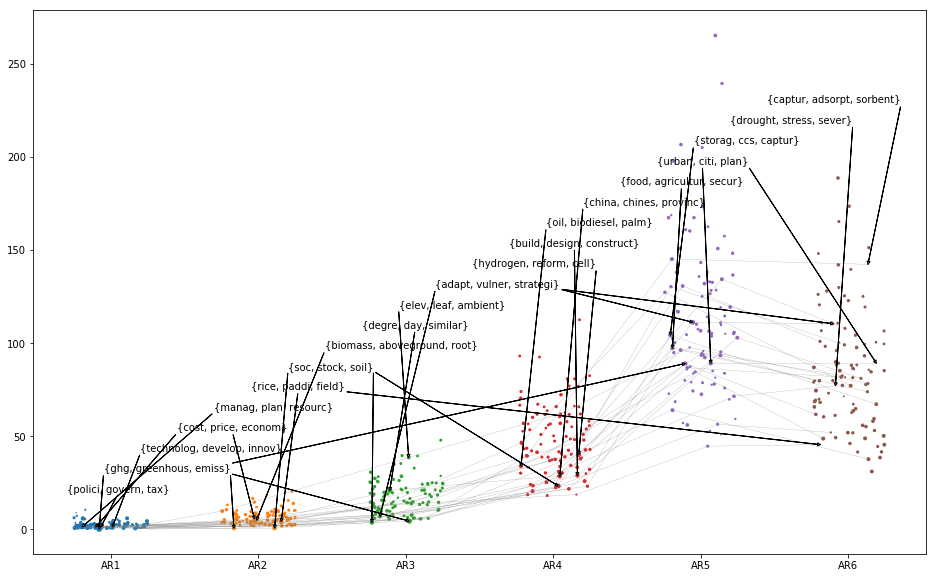
\includegraphics[width=\linewidth]{plots/hot_topics_65}
    \caption{Topic growth over time. The 3 topics in each assessment period that grew by the largest amount are labelled [Example figure]}
    \label{topic_growth}
\end{figure}

\begin{figure}
	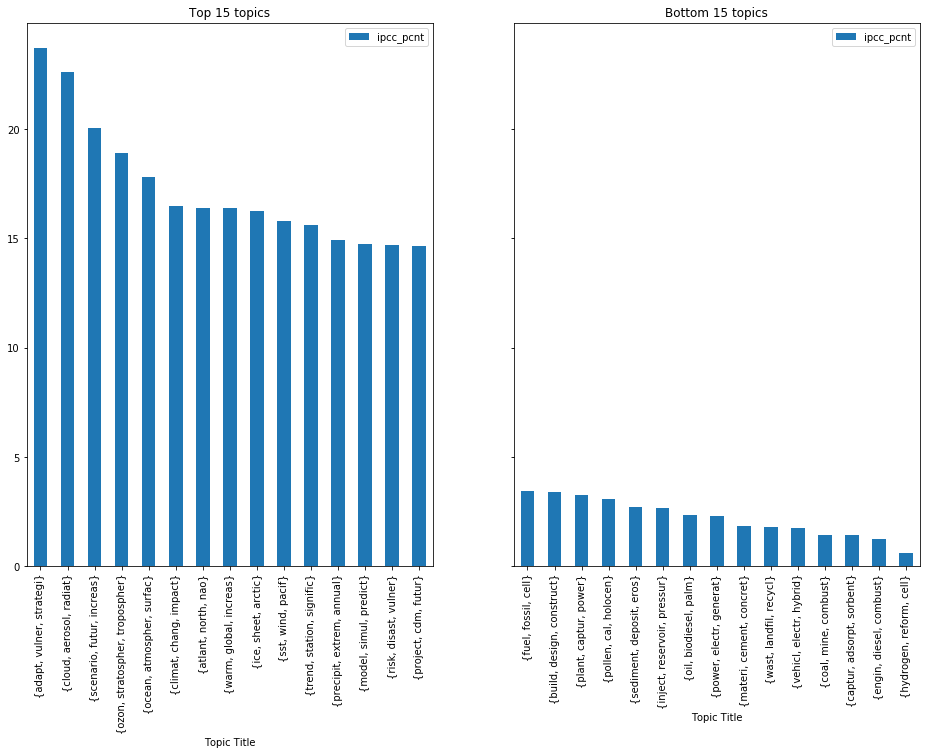
\includegraphics[width=\linewidth]{plots/ipcc_topics_65}
    \caption{IPCC references by topic. The bars show the percentage of each topic that has been matched to an IPCC reference}
    \label{IPCC}
\end{figure}

\begin{table}
\small
\setlength\tabcolsep{0.1cm}
\begin{tabular}{cccccc}
AR1 & AR2 & AR3 & AR4 & AR5 & AR6 \\
\midrule \\
\begin{tabular}{p{2cm}r}
\toprule
                   topic\_\_title &  pchange \\
\midrule
      \{delta, isotop, thousand\} &   40144\% \\
           \{methan, flux, oxid\} &   27808\% \\
            \{model, simul, use\} &   23694\% \\
         \{soil, organ, microbi\} &   23110\% \\
 \{polici, develop, environment\} &   21927\% \\
\bottomrule
\end{tabular}
 & \begin{tabular}{p{1.2cm}r}
\toprule
             topic\_\_title &  pchange \\
\midrule
       \{soc, stock, soil\} &   12638\% \\
    \{fire, burn, wildfir\} &   10893\% \\
    \{coral, reef, bleach\} &    7619\% \\
 \{glacier, mass, retreat\} &    7543\% \\
   \{fuel, vehicl, fossil\} &    4897\% \\
\bottomrule
\end{tabular}
  & \begin{tabular}{p{1.2cm}r}
\toprule
                    title &  pchange \\
\midrule
         soil, soc, organ &     304\% \\
        plant, elev, leaf &     248\% \\
 precipit, rainfal, trend &     235\% \\
      tree, growth, stand &     232\% \\
      adapt, risk, vulner &     231\% \\
\bottomrule
\end{tabular}

 & \begin{tabular}{llr}
\toprule
{} &           topic\_\_title &  pchange \\
\midrule
0 &     \{soc, stock, soil\} &     466\% \\
1 &   \{popul, genet, gene\} &     272\% \\
2 &  \{coral, reef, bleach\} &     232\% \\
3 &   \{flood, risk, event\} &     226\% \\
4 &  \{fire, burn, wildfir\} &     216\% \\
\bottomrule
\end{tabular}
  & \begin{tabular}{p{1.2cm}r}
\toprule
                         title &  pchange \\
\midrule
           adapt, risk, vulner &     320\% \\
             urban, citi, area &     290\% \\
           coral, reef, bleach &     223\% \\
 develop, environment, sustain &     220\% \\
          captur, process, gas &     208\% \\
\bottomrule
\end{tabular}
  & \begin{tabular}{p{1.2cm}r}
\toprule
                    title &  pchange \\
\midrule
   drought, stress, sever &       8\% \\
       rice, paddi, field &       2\% \\
        urban, citi, plan &      -0\% \\
  adapt, vulner, strategi &      -1\% \\
 captur, adsorpt, sorbent &      -2\% \\
\bottomrule
\end{tabular}

\end{tabular}
\caption{The top 5 topics in each assessment period by percentage growth since the last assessment period}
\end{table}

\begin{table}
\small
\setlength\tabcolsep{0.1cm}
\begin{tabular}{cccccc}
AR1 & AR2 & AR3 & AR4 & AR5 & AR6 \\
\midrule \\
\begin{tabular}{p{1.2cm}r}
\toprule
                     title &  pchange \\
\midrule
         tree, stand, ring &     -11\% \\
          soc, stock, soil &     -15\% \\
       coal, mine, combust &     -19\% \\
 dioxid, carbon, atmospher &     -23\% \\
     solar, radiat, irradi &     -31\% \\
\bottomrule
\end{tabular}
 & \begin{tabular}{p{1.2cm}r}
\toprule
                     title &  pchange \\
\midrule
      fish, fisheri, marin &     534\% \\
       delta, valu, isotop &     125\% \\
 litter, decomposit, organ &     nan\% \\
          soc, stock, soil &     nan\% \\
  biochar, amend, pyrolysi &     nan\% \\
\bottomrule
\end{tabular}
  & \begin{tabular}{p{1.2cm}r}
\toprule
                         title &  pchange \\
\midrule
            ice, sheet, arctic &     108\% \\
 ozon, stratospher, tropospher &     103\% \\
       cloud, feedback, radiat &      99\% \\
          fuel, vehicl, fossil &      99\% \\
         warm, global, increas &      94\% \\
\bottomrule
\end{tabular}

 & \begin{tabular}{p{1.2cm}r}
\toprule
                        title &  pchange \\
\midrule
            methan, oxid, gas &      58\% \\
 concentr, atmospher, increas &      54\% \\
           root, respir, fine &      48\% \\
          elev, leaf, ambient &      29\% \\
           rice, paddi, field &      19\% \\
\bottomrule
\end{tabular}
  & \begin{tabular}{p{1.2cm}r}
\toprule
                         title &  pchange \\
\midrule
        cloud, aerosol, radiat &      47\% \\
            ice, sheet, arctic &      45\% \\
              sst, wind, pacif &      42\% \\
            atlant, north, nao &      35\% \\
 ozon, stratospher, tropospher &      25\% \\
\bottomrule
\end{tabular}
  & \begin{tabular}{p{1.2cm}r}
\toprule
                     title &  pchange \\
\midrule
 technolog, develop, innov &     -39\% \\
       coal, mine, combust &     -40\% \\
        fuel, fossil, cell &     -40\% \\
    hydrogen, reform, cell &     -41\% \\
      oil, biodiesel, palm &     -42\% \\
\bottomrule
\end{tabular}

\end{tabular}
\caption{The bottom 5 topics in each assessment period by percentage growth since the last assessment period}
\end{table}

\begin{itemize}
	\item Some big/interesting topics are x and y
	\item These topics have grown at particularly interesting times (Figure \ref{topic_growth})
    \item These topics are better covered in IPCC, these are less well covered \ref{IPCC}
    \item Some interesting topic correlations are x and y; well fitting documents to both include x and y
    \item
\end{itemize}

%\subsection*{Information Retrieval Implications}
%\begin{itemize}
%    \item X keywords fit into Y topics like so...
%    \item Finding similar documents, how does this work with topics as opposed to keywords?
%    \item Similar documents more or less likely to be across disciplinary boundaries ??
%\end{itemize}

\section*{Conclusion}
\begin{itemize}
	\item A very simple topic model provides an overview of the whole landscape.
    \item This allows researchers / assessment makers to identify areas that have grown recently
    \item Topic models aid document discovery, have the potential to contribute to more comprehensive assessments.
	\item AR5 seemed to have less comprehensive coverage of x topics. This was a particular issue in WG y.
	\item This may not be an issue, there could be good reasons for this, but these should be made transparent.
	\item For the next assessment report, x topics may require particular attention.
	\item The emerging topic on CCS resonates with a growing recognition of the importance of negative emissions and the lack of understanding about how they could fill their role. This will be of particular importance for the IPCC special report on 1.5 degrees.
    %\item Next steps for research: using topic models to assess the assessment process: more thorough gapfinding etc.
\end{itemize}




\begin{figure}
	%\includegraphics{}
    \caption{Focus on [biochar?] showing document with highlighted words}
\end{figure}

\begin{figure}
	%\includegraphics{}
    \caption{Model validation graph, showing error for different topic numbers, feature numbers}
\end{figure}


\begin{figure}
	%\includegraphics{}
    \caption{Some relation of topics to other features of dataset: e.g. most interdisciplinary journals and least, or so...}
\end{figure}


\section*{Methodology}

\begin{itemize}
\item Topic modelling in general: reducing large matrix of documents to words to two smaller matrices of topics x words and topics x documents.
\item Model selection: NMF \citep{Lee1999}
\item How does it work? Advantages: Simple, scalable: better results than with other solutions%, if only because it was possible to iterate with large document collections. LDA can be better but relies on tuning hyperparameters, hard to do with such big corpus
\item Topic model browser \citet{Chaney2012}
\item Merging with IPCC citation dataset - caveats...
\item Network explanation
\item Regression of network score on dummy variable for same
%\item Compare topic space to keyword space. Reduces dimensionality, overcomes non-standardisation
%\item Which topics get the most citations?

\end{itemize}

\section{Data}
\begin{itemize}
	\item Queries: use \citet{Grieneisen2011}, or take the best bits of \citet{Grieneisen2011} and \citet{Haunschild2016}?
    \item Sources: WoS, Scopus or both?
    \item Preprocessing: Remove punctuation, numbers, common, uncommon words, stemming
\end{itemize}





\listoffigures
\linespread{1}
\bibliography{Mendeley.bib}
\bibliographystyle{apalike}

\end{document}

